\documentclass[twoside]{book}

% Packages required by doxygen
\usepackage{fixltx2e}
\usepackage{calc}
\usepackage{doxygen}
\usepackage[export]{adjustbox} % also loads graphicx
\usepackage{graphicx}
\usepackage[utf8]{inputenc}
\usepackage{makeidx}
\usepackage{multicol}
\usepackage{multirow}
\PassOptionsToPackage{warn}{textcomp}
\usepackage{textcomp}
\usepackage[nointegrals]{wasysym}
\usepackage[table]{xcolor}

% Font selection
\usepackage[T1]{fontenc}
\usepackage[scaled=.90]{helvet}
\usepackage{courier}
\usepackage{amssymb}
\usepackage{sectsty}
\renewcommand{\familydefault}{\sfdefault}
\allsectionsfont{%
  \fontseries{bc}\selectfont%
  \color{darkgray}%
}
\renewcommand{\DoxyLabelFont}{%
  \fontseries{bc}\selectfont%
  \color{darkgray}%
}
\newcommand{\+}{\discretionary{\mbox{\scriptsize$\hookleftarrow$}}{}{}}

% Page & text layout
\usepackage{geometry}
\geometry{%
  a4paper,%
  top=2.5cm,%
  bottom=2.5cm,%
  left=2.5cm,%
  right=2.5cm%
}
\tolerance=750
\hfuzz=15pt
\hbadness=750
\setlength{\emergencystretch}{15pt}
\setlength{\parindent}{0cm}
\setlength{\parskip}{3ex plus 2ex minus 2ex}
\makeatletter
\renewcommand{\paragraph}{%
  \@startsection{paragraph}{4}{0ex}{-1.0ex}{1.0ex}{%
    \normalfont\normalsize\bfseries\SS@parafont%
  }%
}
\renewcommand{\subparagraph}{%
  \@startsection{subparagraph}{5}{0ex}{-1.0ex}{1.0ex}{%
    \normalfont\normalsize\bfseries\SS@subparafont%
  }%
}
\makeatother

% Headers & footers
\usepackage{fancyhdr}
\pagestyle{fancyplain}
\fancyhead[LE]{\fancyplain{}{\bfseries\thepage}}
\fancyhead[CE]{\fancyplain{}{}}
\fancyhead[RE]{\fancyplain{}{\bfseries\leftmark}}
\fancyhead[LO]{\fancyplain{}{\bfseries\rightmark}}
\fancyhead[CO]{\fancyplain{}{}}
\fancyhead[RO]{\fancyplain{}{\bfseries\thepage}}
\fancyfoot[LE]{\fancyplain{}{}}
\fancyfoot[CE]{\fancyplain{}{}}
\fancyfoot[RE]{\fancyplain{}{\bfseries\scriptsize Generated by Doxygen }}
\fancyfoot[LO]{\fancyplain{}{\bfseries\scriptsize Generated by Doxygen }}
\fancyfoot[CO]{\fancyplain{}{}}
\fancyfoot[RO]{\fancyplain{}{}}
\renewcommand{\footrulewidth}{0.4pt}
\renewcommand{\chaptermark}[1]{%
  \markboth{#1}{}%
}
\renewcommand{\sectionmark}[1]{%
  \markright{\thesection\ #1}%
}

% Indices & bibliography
\usepackage{natbib}
\usepackage[titles]{tocloft}
\setcounter{tocdepth}{3}
\setcounter{secnumdepth}{5}
\makeindex

% Hyperlinks (required, but should be loaded last)
\usepackage{ifpdf}
\ifpdf
  \usepackage[pdftex,pagebackref=true]{hyperref}
\else
  \usepackage[ps2pdf,pagebackref=true]{hyperref}
\fi
\hypersetup{%
  colorlinks=true,%
  linkcolor=blue,%
  citecolor=blue,%
  unicode%
}

% Custom commands
\newcommand{\clearemptydoublepage}{%
  \newpage{\pagestyle{empty}\cleardoublepage}%
}

\usepackage{caption}
\captionsetup{labelsep=space,justification=centering,font={bf},singlelinecheck=off,skip=4pt,position=top}

%===== C O N T E N T S =====

\begin{document}

% Titlepage & ToC
\hypersetup{pageanchor=false,
             bookmarksnumbered=true,
             pdfencoding=unicode
            }
\pagenumbering{roman}
\begin{titlepage}
\vspace*{7cm}
\begin{center}%
{\Large barn\+\_\+test }\\
\vspace*{1cm}
{\large Generated by Doxygen 1.8.11}\\
\end{center}
\end{titlepage}
\clearemptydoublepage
\tableofcontents
\clearemptydoublepage
\pagenumbering{arabic}
\hypersetup{pageanchor=true}

%--- Begin generated contents ---
\chapter{Main Page}
\label{index}\hypertarget{index}{}The barn\+\_\+test package provides simple, portable small-\/scale tools for unit testing.

Dont be shy to look into the sources for further direct information. 
\chapter{Namespace Index}
\section{Namespace List}
Here is a list of all documented namespaces with brief descriptions\+:\begin{DoxyCompactList}
\item\contentsline{section}{\hyperlink{namespaceunittest_1_1tuple__to__stream_1_1detail}{unittest\+::tuple\+\_\+to\+\_\+stream\+::detail} \\*Implementation details, clients never use these directly }{\pageref{namespaceunittest_1_1tuple__to__stream_1_1detail}}{}
\end{DoxyCompactList}

\chapter{Hierarchical Index}
\section{Class Hierarchy}
This inheritance list is sorted roughly, but not completely, alphabetically\+:\begin{DoxyCompactList}
\item \contentsline{section}{unittest\+:\+:Randomized\+Function\+Test$<$ Result\+Type, Arg\+Types $>$\+:\+:Error\+Case\+Type}{\pageref{structunittest_1_1_randomized_function_test_1_1_error_case_type}}{}
\item \contentsline{section}{unittest\+:\+:Function\+Test$<$ Result\+Type, Arg\+Types $>$}{\pageref{classunittest_1_1_function_test}}{}
\item \contentsline{section}{unittest\+:\+:tuple\+\_\+to\+\_\+stream\+:\+:detail\+:\+:gen\+\_\+seq$<$ N, Is $>$}{\pageref{structunittest_1_1tuple__to__stream_1_1detail_1_1gen__seq}}{}
\item \contentsline{section}{unittest\+:\+:Randomized\+Function\+Test$<$ Result\+Type, Arg\+Types $>$}{\pageref{classunittest_1_1_randomized_function_test}}{}
\item \contentsline{section}{unittest\+:\+:tuple\+\_\+to\+\_\+stream\+:\+:detail\+:\+:seq$<$... $>$}{\pageref{structunittest_1_1tuple__to__stream_1_1detail_1_1seq}}{}
\item \contentsline{section}{unittest\+:\+:tuple\+\_\+to\+\_\+stream\+:\+:detail\+:\+:seq$<$ Is... $>$}{\pageref{structunittest_1_1tuple__to__stream_1_1detail_1_1seq}}{}
\begin{DoxyCompactList}
\item \contentsline{section}{unittest\+:\+:tuple\+\_\+to\+\_\+stream\+:\+:detail\+:\+:gen\+\_\+seq$<$ 0, Is... $>$}{\pageref{structunittest_1_1tuple__to__stream_1_1detail_1_1gen__seq_3_010_00_01_is_8_8_8_01_4}}{}
\end{DoxyCompactList}
\item \contentsline{section}{unittest\+:\+:Randomized\+Function\+Test$<$ Result\+Type, Arg\+Types $>$\+:\+:Test\+Return\+Type}{\pageref{structunittest_1_1_randomized_function_test_1_1_test_return_type}}{}
\item \contentsline{section}{unittest\+:\+:Function\+Test$<$ Result\+Type, Arg\+Types $>$\+:\+:Test\+Return\+Type}{\pageref{structunittest_1_1_function_test_1_1_test_return_type}}{}
\end{DoxyCompactList}

\chapter{Class Index}
\section{Class List}
Here are the classes, structs, unions and interfaces with brief descriptions\+:\begin{DoxyCompactList}
\item\contentsline{section}{\hyperlink{classunittest_1_1_function_test}{unittest\+::\+Function\+Test$<$ Result\+Type, Arg\+Types $>$} }{\pageref{classunittest_1_1_function_test}}{}
\end{DoxyCompactList}

\chapter{Namespace Documentation}
\hypertarget{namespaceunittest_1_1tuple__to__stream_1_1detail}{}\section{unittest\+:\+:tuple\+\_\+to\+\_\+stream\+:\+:detail Namespace Reference}
\label{namespaceunittest_1_1tuple__to__stream_1_1detail}\index{unittest\+::tuple\+\_\+to\+\_\+stream\+::detail@{unittest\+::tuple\+\_\+to\+\_\+stream\+::detail}}


Implementation details, clients never use these directly.  


\subsection*{Classes}
\begin{DoxyCompactItemize}
\item 
struct \hyperlink{structunittest_1_1tuple__to__stream_1_1detail_1_1gen__seq}{gen\+\_\+seq}
\item 
struct \hyperlink{structunittest_1_1tuple__to__stream_1_1detail_1_1gen__seq_3_010_00_01_is_8_8_8_01_4}{gen\+\_\+seq$<$ 0, Is... $>$}
\item 
struct \hyperlink{structunittest_1_1tuple__to__stream_1_1detail_1_1seq}{seq}
\begin{DoxyCompactList}\small\item\em Implementation details, clients never use these directly. \end{DoxyCompactList}\end{DoxyCompactItemize}
\subsection*{Functions}
\begin{DoxyCompactItemize}
\item 
{\footnotesize template$<$class Ch , class Tr , class Tuple , std\+::size\+\_\+t... Is$>$ }\\std\+::basic\+\_\+ostream$<$ Ch, Tr $>$ \& {\bfseries to\+\_\+stream} (std\+::basic\+\_\+ostream$<$ Ch, Tr $>$ \&os, Tuple const \&t, \hyperlink{structunittest_1_1tuple__to__stream_1_1detail_1_1seq}{seq}$<$ Is... $>$)\hypertarget{namespaceunittest_1_1tuple__to__stream_1_1detail_a5ae468d1bc1a9bfada84010996bc3bef}{}\label{namespaceunittest_1_1tuple__to__stream_1_1detail_a5ae468d1bc1a9bfada84010996bc3bef}

\end{DoxyCompactItemize}


\subsection{Detailed Description}
Implementation details, clients never use these directly. 
\chapter{Class Documentation}
\hypertarget{structunittest_1_1_randomized_function_test_1_1_error_case_type}{}\section{unittest\+:\+:Randomized\+Function\+Test$<$ Result\+Type, Arg\+Types $>$\+:\+:Error\+Case\+Type Struct Reference}
\label{structunittest_1_1_randomized_function_test_1_1_error_case_type}\index{unittest\+::\+Randomized\+Function\+Test$<$ Result\+Type, Arg\+Types $>$\+::\+Error\+Case\+Type@{unittest\+::\+Randomized\+Function\+Test$<$ Result\+Type, Arg\+Types $>$\+::\+Error\+Case\+Type}}


Stores information on the circumstances which cause a single test to fail.  




{\ttfamily \#include $<$Randomized\+Function\+Test.\+hpp$>$}

\subsection*{Public Attributes}
\begin{DoxyCompactItemize}
\item 
Result\+Type \hyperlink{structunittest_1_1_randomized_function_test_1_1_error_case_type_aac3651b4656294eb6dfa1f8997936685}{erroneous\+\_\+result}\hypertarget{structunittest_1_1_randomized_function_test_1_1_error_case_type_aac3651b4656294eb6dfa1f8997936685}{}\label{structunittest_1_1_randomized_function_test_1_1_error_case_type_aac3651b4656294eb6dfa1f8997936685}

\begin{DoxyCompactList}\small\item\em The errorneous function return value. \end{DoxyCompactList}\item 
Result\+Type \hyperlink{structunittest_1_1_randomized_function_test_1_1_error_case_type_a15a54a6d7304321aae4b838e3d95b57a}{reference\+\_\+result}\hypertarget{structunittest_1_1_randomized_function_test_1_1_error_case_type_a15a54a6d7304321aae4b838e3d95b57a}{}\label{structunittest_1_1_randomized_function_test_1_1_error_case_type_a15a54a6d7304321aae4b838e3d95b57a}

\begin{DoxyCompactList}\small\item\em The supposedly correct return value of the reference function. \end{DoxyCompactList}\item 
Args\+Tuple\+Type \hyperlink{structunittest_1_1_randomized_function_test_1_1_error_case_type_a42a56dc7973866d25db122de90c69173}{args}\hypertarget{structunittest_1_1_randomized_function_test_1_1_error_case_type_a42a56dc7973866d25db122de90c69173}{}\label{structunittest_1_1_randomized_function_test_1_1_error_case_type_a42a56dc7973866d25db122de90c69173}

\begin{DoxyCompactList}\small\item\em The corresponding function invocation arguments. \end{DoxyCompactList}\end{DoxyCompactItemize}


\subsection{Detailed Description}
\subsubsection*{template$<$typename Result\+Type, typename... Arg\+Types$>$\\*
struct unittest\+::\+Randomized\+Function\+Test$<$ Result\+Type, Arg\+Types $>$\+::\+Error\+Case\+Type}

Stores information on the circumstances which cause a single test to fail. 

The documentation for this struct was generated from the following file\+:\begin{DoxyCompactItemize}
\item 
D\+:/\+Dev/\+\_\+\+Lib/barn\+\_\+test/Randomized\+Function\+Test.\+hpp\end{DoxyCompactItemize}

\hypertarget{classunittest_1_1_function_test}{}\section{unittest\+:\+:Function\+Test$<$ Result\+Type, Arg\+Types $>$ Class Template Reference}
\label{classunittest_1_1_function_test}\index{unittest\+::\+Function\+Test$<$ Result\+Type, Arg\+Types $>$@{unittest\+::\+Function\+Test$<$ Result\+Type, Arg\+Types $>$}}


{\ttfamily \#include $<$Function\+Test.\+hpp$>$}

\subsection*{Public Member Functions}
\begin{DoxyCompactItemize}
\item 
\hyperlink{classunittest_1_1_function_test_a9bb46bed56452a5354848e7d5744c715}{Function\+Test} (Function\+Type function, Comparator\+Function\+Type comparator, To\+String\+Function\+Type to\+\_\+string\+\_\+function, std\+::ostream \&os=std\+::cout)
\item 
\hyperlink{classunittest_1_1_function_test_addafa5fd128998c358ef14732d4afeb0}{Function\+Test} (Function\+Type function, Comparator\+Function\+Type comparator, std\+::ostream \&os=std\+::cout)
\item 
\hyperlink{classunittest_1_1_function_test_a27a92d51dc33cdd08f025555b3d73de8}{Function\+Test} (Function\+Type function, std\+::ostream \&os=std\+::cout)
\item 
{\footnotesize template$<$typename T $>$ }\\std\+::pair$<$ bool, Result\+Type $>$ \hyperlink{classunittest_1_1_function_test_abd6a6fe7f829fbedb7fdec63a61ed122}{test} (const std\+::string \&, const T \&, const Arg\+Types \&...) const  =delete
\item 
Test\+Return\+Type \hyperlink{classunittest_1_1_function_test_adeb82aea0d7e1975da9f55d5170d31d6}{test} (const std\+::string \&test\+\_\+name, const Result\+Type \&expected\+\_\+result, const Arg\+Types \&...args)
\item 
bool \hyperlink{classunittest_1_1_function_test_a1263b315394a9d4d8bf2a7f5e66be9c6}{write\+\_\+test\+\_\+series\+\_\+summary} () const 
\item 
unsigned int \hyperlink{classunittest_1_1_function_test_a377bc6b2de27ae65ca82f7f063691745}{n\+\_\+tests} () const \hypertarget{classunittest_1_1_function_test_a377bc6b2de27ae65ca82f7f063691745}{}\label{classunittest_1_1_function_test_a377bc6b2de27ae65ca82f7f063691745}

\begin{DoxyCompactList}\small\item\em Returns the number of tests. \end{DoxyCompactList}\item 
unsigned int \hyperlink{classunittest_1_1_function_test_acc025a166bf4840d426e2a9f0b639297}{n\+\_\+passed\+\_\+tests} () const \hypertarget{classunittest_1_1_function_test_acc025a166bf4840d426e2a9f0b639297}{}\label{classunittest_1_1_function_test_acc025a166bf4840d426e2a9f0b639297}

\begin{DoxyCompactList}\small\item\em Returns the number of passed tests. \end{DoxyCompactList}\item 
bool \hyperlink{classunittest_1_1_function_test_a986ab165971bbf218117ef36a9b6cda0}{is\+\_\+last\+\_\+test\+\_\+passed} () const \hypertarget{classunittest_1_1_function_test_a986ab165971bbf218117ef36a9b6cda0}{}\label{classunittest_1_1_function_test_a986ab165971bbf218117ef36a9b6cda0}

\begin{DoxyCompactList}\small\item\em Returns if the last test whas passed. Also returns T\+R\+UE if no test was executed. \end{DoxyCompactList}\item 
Test\+Duration\+Type \hyperlink{classunittest_1_1_function_test_a63136c98f5f9f8189ff710112bd55a08}{last\+\_\+invocation\+\_\+duration} () const \hypertarget{classunittest_1_1_function_test_a63136c98f5f9f8189ff710112bd55a08}{}\label{classunittest_1_1_function_test_a63136c98f5f9f8189ff710112bd55a08}

\begin{DoxyCompactList}\small\item\em The duration of the last function invocation. \end{DoxyCompactList}\item 
Result\+Type \hyperlink{classunittest_1_1_function_test_acd04aafd9cb3bb7ee22876e1e3979a11}{last\+\_\+test\+\_\+result} () const \hypertarget{classunittest_1_1_function_test_acd04aafd9cb3bb7ee22876e1e3979a11}{}\label{classunittest_1_1_function_test_acd04aafd9cb3bb7ee22876e1e3979a11}

\begin{DoxyCompactList}\small\item\em Returns a assignment-\/copy of the result of the last test. \end{DoxyCompactList}\item 
bool \hyperlink{classunittest_1_1_function_test_ac54d10d4dba64b9545ae7b2d30ae3d48}{is\+\_\+all\+\_\+tests\+\_\+passed} () const \hypertarget{classunittest_1_1_function_test_ac54d10d4dba64b9545ae7b2d30ae3d48}{}\label{classunittest_1_1_function_test_ac54d10d4dba64b9545ae7b2d30ae3d48}

\begin{DoxyCompactList}\small\item\em Indicates whether every test so far passed or not. Also returns T\+R\+UE if no test was executed. \end{DoxyCompactList}\item 
Test\+Duration\+Type \hyperlink{classunittest_1_1_function_test_a09ae97b06e34d144f243dcef00ead1a9}{accumulated\+\_\+invocation\+\_\+durations} () const \hypertarget{classunittest_1_1_function_test_a09ae97b06e34d144f243dcef00ead1a9}{}\label{classunittest_1_1_function_test_a09ae97b06e34d144f243dcef00ead1a9}

\begin{DoxyCompactList}\small\item\em The accumulated execution time for all function invocations. \end{DoxyCompactList}\end{DoxyCompactItemize}
\subsection*{Public Attributes}
\begin{DoxyCompactItemize}
\item 
bool \hyperlink{classunittest_1_1_function_test_a0eb2680ff0867ff55daffa2b09c90280}{verbose} = true\hypertarget{classunittest_1_1_function_test_a0eb2680ff0867ff55daffa2b09c90280}{}\label{classunittest_1_1_function_test_a0eb2680ff0867ff55daffa2b09c90280}

\begin{DoxyCompactList}\small\item\em Whether or not show detailed info in case of failures. \end{DoxyCompactList}\item 
unsigned int \hyperlink{classunittest_1_1_function_test_aa9959c19872e086b9401382cb381f552}{output\+\_\+line\+\_\+length} = 60\hypertarget{classunittest_1_1_function_test_aa9959c19872e086b9401382cb381f552}{}\label{classunittest_1_1_function_test_aa9959c19872e086b9401382cb381f552}

\begin{DoxyCompactList}\small\item\em The number of dots that is shown in the printed lines. \end{DoxyCompactList}\end{DoxyCompactItemize}


\subsection{Detailed Description}
\subsubsection*{template$<$typename Result\+Type, typename... Arg\+Types$>$\\*
class unittest\+::\+Function\+Test$<$ Result\+Type, Arg\+Types $>$}

\hyperlink{classunittest_1_1_function_test}{Function\+Test} unit testing class wich is capable of invoking arbitrary functions with a return value and comparing them to anticipated values. Measures the run-\/time of the function and writes unit test results to a stream. 

\subsection{Constructor \& Destructor Documentation}
\index{unittest\+::\+Function\+Test@{unittest\+::\+Function\+Test}!Function\+Test@{Function\+Test}}
\index{Function\+Test@{Function\+Test}!unittest\+::\+Function\+Test@{unittest\+::\+Function\+Test}}
\subsubsection[{\texorpdfstring{Function\+Test(\+Function\+Type function, Comparator\+Function\+Type comparator, To\+String\+Function\+Type to\+\_\+string\+\_\+function, std\+::ostream \&os=std\+::cout)}{FunctionTest(FunctionType function, ComparatorFunctionType comparator, ToStringFunctionType to_string_function, std::ostream &os=std::cout)}}]{\setlength{\rightskip}{0pt plus 5cm}template$<$typename Result\+Type , typename... Arg\+Types$>$ {\bf unittest\+::\+Function\+Test}$<$ Result\+Type, Arg\+Types $>$\+::{\bf Function\+Test} (
\begin{DoxyParamCaption}
\item[{Function\+Type}]{function, }
\item[{Comparator\+Function\+Type}]{comparator, }
\item[{To\+String\+Function\+Type}]{to\+\_\+string\+\_\+function, }
\item[{std\+::ostream \&}]{os = {\ttfamily std\+:\+:cout}}
\end{DoxyParamCaption}
)\hspace{0.3cm}{\ttfamily [inline]}}\hypertarget{classunittest_1_1_function_test_a9bb46bed56452a5354848e7d5744c715}{}\label{classunittest_1_1_function_test_a9bb46bed56452a5354848e7d5744c715}
Constructor \#1 for the function tester. Use with complex return types. Sets the verbose flag to T\+R\+UE. 
\begin{DoxyParams}{Parameters}
{\em function} & A function that must return a value. \\
\hline
{\em comparator} & A comparison function that compares the actual invocation-\/results with given expected results. The comparison function must have the form bool(\+Result\+Type, Result\+Type) or similar. \\
\hline
{\em to\+\_\+string\+\_\+function} & The to-\/string function for the function\textquotesingle{}s return type. \\
\hline
{\em os} & An ostream to which the output is streamed. \\
\hline
\end{DoxyParams}
\index{unittest\+::\+Function\+Test@{unittest\+::\+Function\+Test}!Function\+Test@{Function\+Test}}
\index{Function\+Test@{Function\+Test}!unittest\+::\+Function\+Test@{unittest\+::\+Function\+Test}}
\subsubsection[{\texorpdfstring{Function\+Test(\+Function\+Type function, Comparator\+Function\+Type comparator, std\+::ostream \&os=std\+::cout)}{FunctionTest(FunctionType function, ComparatorFunctionType comparator, std::ostream &os=std::cout)}}]{\setlength{\rightskip}{0pt plus 5cm}template$<$typename Result\+Type , typename... Arg\+Types$>$ {\bf unittest\+::\+Function\+Test}$<$ Result\+Type, Arg\+Types $>$\+::{\bf Function\+Test} (
\begin{DoxyParamCaption}
\item[{Function\+Type}]{function, }
\item[{Comparator\+Function\+Type}]{comparator, }
\item[{std\+::ostream \&}]{os = {\ttfamily std\+:\+:cout}}
\end{DoxyParamCaption}
)\hspace{0.3cm}{\ttfamily [inline]}}\hypertarget{classunittest_1_1_function_test_addafa5fd128998c358ef14732d4afeb0}{}\label{classunittest_1_1_function_test_addafa5fd128998c358ef14732d4afeb0}
Constructor \#2 for the function tester. Use with complex return types. Sets the to-\/string function for the function\textquotesingle{}s return type to a standard function and sets the verbose flag to F\+A\+L\+SE. 
\begin{DoxyParams}{Parameters}
{\em function} & A function that must return a value. \\
\hline
{\em comparator} & A comparison function that compares the actual invocation-\/results with given expected results. The comparison function must have the form bool(\+Result\+Type, Result\+Type) or similar. \\
\hline
{\em os} & An ostream to which the output is streamed. \\
\hline
\end{DoxyParams}
\index{unittest\+::\+Function\+Test@{unittest\+::\+Function\+Test}!Function\+Test@{Function\+Test}}
\index{Function\+Test@{Function\+Test}!unittest\+::\+Function\+Test@{unittest\+::\+Function\+Test}}
\subsubsection[{\texorpdfstring{Function\+Test(\+Function\+Type function, std\+::ostream \&os=std\+::cout)}{FunctionTest(FunctionType function, std::ostream &os=std::cout)}}]{\setlength{\rightskip}{0pt plus 5cm}template$<$typename Result\+Type , typename... Arg\+Types$>$ {\bf unittest\+::\+Function\+Test}$<$ Result\+Type, Arg\+Types $>$\+::{\bf Function\+Test} (
\begin{DoxyParamCaption}
\item[{Function\+Type}]{function, }
\item[{std\+::ostream \&}]{os = {\ttfamily std\+:\+:cout}}
\end{DoxyParamCaption}
)\hspace{0.3cm}{\ttfamily [inline]}}\hypertarget{classunittest_1_1_function_test_a27a92d51dc33cdd08f025555b3d73de8}{}\label{classunittest_1_1_function_test_a27a92d51dc33cdd08f025555b3d73de8}
Constructor \#3 for the function tester. Use with simple return types. Sets the comparison function to a simple \char`\"{}==\char`\"{}. Sets the to-\/string function for the function\textquotesingle{}s return type to a standard function and sets the verbose flag to T\+R\+UE. 
\begin{DoxyParams}{Parameters}
{\em function} & A function that must return a value. \\
\hline
{\em os} & An ostream to which the output is streamed. \\
\hline
\end{DoxyParams}


\subsection{Member Function Documentation}
\index{unittest\+::\+Function\+Test@{unittest\+::\+Function\+Test}!test@{test}}
\index{test@{test}!unittest\+::\+Function\+Test@{unittest\+::\+Function\+Test}}
\subsubsection[{\texorpdfstring{test(const std\+::string \&, const T \&, const Arg\+Types \&...) const  =delete}{test(const std::string &, const T &, const ArgTypes &...) const  =delete}}]{\setlength{\rightskip}{0pt plus 5cm}template$<$typename Result\+Type , typename... Arg\+Types$>$ template$<$typename T $>$ std\+::pair$<$bool, Result\+Type$>$ {\bf unittest\+::\+Function\+Test}$<$ Result\+Type, Arg\+Types $>$\+::test (
\begin{DoxyParamCaption}
\item[{const std\+::string \&}]{, }
\item[{const T \&}]{, }
\item[{const Arg\+Types \&}]{...}
\end{DoxyParamCaption}
) const\hspace{0.3cm}{\ttfamily [delete]}}\hypertarget{classunittest_1_1_function_test_abd6a6fe7f829fbedb7fdec63a61ed122}{}\label{classunittest_1_1_function_test_abd6a6fe7f829fbedb7fdec63a61ed122}
This deleted function prevents callers from handing expected result of wrong type. This prevents false negatives through conversion errors, like double to int truncation. Consider a test on a function int()\{ return 1 \}\+: tester.\+test(\char`\"{}1\char`\"{}, 1.\+2); won\textquotesingle{}t compile (otherwise, it would convert to 1 which then yielded OK) tester.\+test(\char`\"{}2\char`\"{}, 1); compiles. \index{unittest\+::\+Function\+Test@{unittest\+::\+Function\+Test}!test@{test}}
\index{test@{test}!unittest\+::\+Function\+Test@{unittest\+::\+Function\+Test}}
\subsubsection[{\texorpdfstring{test(const std\+::string \&test\+\_\+name, const Result\+Type \&expected\+\_\+result, const Arg\+Types \&...\+args)}{test(const std::string &test_name, const ResultType &expected_result, const ArgTypes &...args)}}]{\setlength{\rightskip}{0pt plus 5cm}template$<$typename Result\+Type , typename... Arg\+Types$>$ Test\+Return\+Type {\bf unittest\+::\+Function\+Test}$<$ Result\+Type, Arg\+Types $>$\+::test (
\begin{DoxyParamCaption}
\item[{const std\+::string \&}]{test\+\_\+name, }
\item[{const Result\+Type \&}]{expected\+\_\+result, }
\item[{const Arg\+Types \&...}]{args}
\end{DoxyParamCaption}
)\hspace{0.3cm}{\ttfamily [inline]}}\hypertarget{classunittest_1_1_function_test_adeb82aea0d7e1975da9f55d5170d31d6}{}\label{classunittest_1_1_function_test_adeb82aea0d7e1975da9f55d5170d31d6}
Unit test on the function that is connected to the tester. Tests whether the return-\/value of a given function invoked with given parameters is equal to a given value and takes care of possibly occuring exceptions. Also measures the time the function execution takes and writes the results of the test to a given output-\/stream. Checks also for exceptions and reports them to the output stream. In case of error the object\textquotesingle{}s flag .verbose in conjunction with a valid .result\+\_\+to\+\_\+string\+\_\+function can be used to write more sophisticated output. 
\begin{DoxyParams}{Parameters}
{\em test\+\_\+name} & A human-\/readable alias of the test that will be written into the stream. \\
\hline
{\em expected\+\_\+result} & The anticipated return value of the tested function. \\
\hline
{\em args} & The arguments that will be passed to the function on invocation. \\
\hline
\end{DoxyParams}
\begin{DoxyReturn}{Returns}
A pair$<$bool, Result\+Type$>$. The first value represents whether the test was successful or not. The second value is a copy of the actual result of the function invocation. 
\end{DoxyReturn}
\index{unittest\+::\+Function\+Test@{unittest\+::\+Function\+Test}!write\+\_\+test\+\_\+series\+\_\+summary@{write\+\_\+test\+\_\+series\+\_\+summary}}
\index{write\+\_\+test\+\_\+series\+\_\+summary@{write\+\_\+test\+\_\+series\+\_\+summary}!unittest\+::\+Function\+Test@{unittest\+::\+Function\+Test}}
\subsubsection[{\texorpdfstring{write\+\_\+test\+\_\+series\+\_\+summary() const }{write_test_series_summary() const }}]{\setlength{\rightskip}{0pt plus 5cm}template$<$typename Result\+Type , typename... Arg\+Types$>$ bool {\bf unittest\+::\+Function\+Test}$<$ Result\+Type, Arg\+Types $>$\+::write\+\_\+test\+\_\+series\+\_\+summary (
\begin{DoxyParamCaption}
{}
\end{DoxyParamCaption}
) const\hspace{0.3cm}{\ttfamily [inline]}}\hypertarget{classunittest_1_1_function_test_a1263b315394a9d4d8bf2a7f5e66be9c6}{}\label{classunittest_1_1_function_test_a1263b315394a9d4d8bf2a7f5e66be9c6}
After running a series of \hyperlink{classunittest_1_1_function_test_abd6a6fe7f829fbedb7fdec63a61ed122}{Function\+Test\+::test()} invocations, this method can be called to write summarized information to the output stream. \begin{DoxyReturn}{Returns}
T\+R\+UE if all tests until now are passed or no test has been executed. F\+A\+L\+SE otherwise. 
\end{DoxyReturn}


The documentation for this class was generated from the following file\+:\begin{DoxyCompactItemize}
\item 
D\+:/\+Dev/\+\_\+\+Lib/barn\+\_\+test/Function\+Test.\+hpp\end{DoxyCompactItemize}

\hypertarget{structunittest_1_1tuple__to__stream_1_1detail_1_1gen__seq}{}\section{unittest\+:\+:tuple\+\_\+to\+\_\+stream\+:\+:detail\+:\+:gen\+\_\+seq$<$ N, Is $>$ Struct Template Reference}
\label{structunittest_1_1tuple__to__stream_1_1detail_1_1gen__seq}\index{unittest\+::tuple\+\_\+to\+\_\+stream\+::detail\+::gen\+\_\+seq$<$ N, Is $>$@{unittest\+::tuple\+\_\+to\+\_\+stream\+::detail\+::gen\+\_\+seq$<$ N, Is $>$}}


The documentation for this struct was generated from the following file\+:\begin{DoxyCompactItemize}
\item 
D\+:/\+Dev/\+\_\+\+Lib/barn\+\_\+test/tuple\+\_\+to\+\_\+stream.\+hpp\end{DoxyCompactItemize}

\hypertarget{structunittest_1_1tuple__to__stream_1_1detail_1_1gen__seq_3_010_00_01_is_8_8_8_01_4}{}\section{unittest\+:\+:tuple\+\_\+to\+\_\+stream\+:\+:detail\+:\+:gen\+\_\+seq$<$ 0, Is... $>$ Struct Template Reference}
\label{structunittest_1_1tuple__to__stream_1_1detail_1_1gen__seq_3_010_00_01_is_8_8_8_01_4}\index{unittest\+::tuple\+\_\+to\+\_\+stream\+::detail\+::gen\+\_\+seq$<$ 0, Is... $>$@{unittest\+::tuple\+\_\+to\+\_\+stream\+::detail\+::gen\+\_\+seq$<$ 0, Is... $>$}}
Inheritance diagram for unittest\+:\+:tuple\+\_\+to\+\_\+stream\+:\+:detail\+:\+:gen\+\_\+seq$<$ 0, Is... $>$\+:\begin{figure}[H]
\begin{center}
\leavevmode
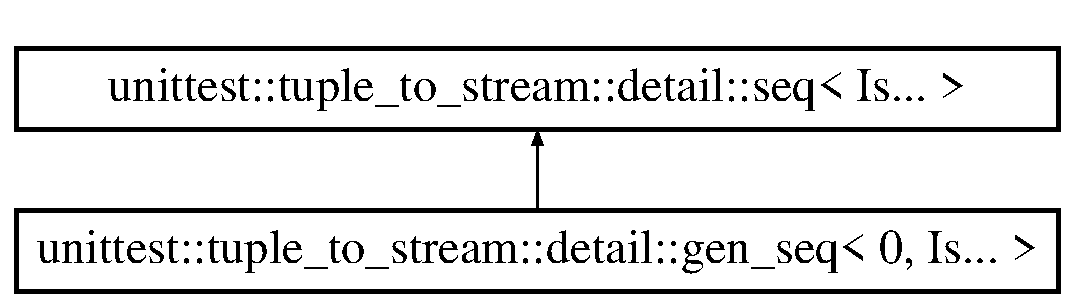
\includegraphics[height=2.000000cm]{structunittest_1_1tuple__to__stream_1_1detail_1_1gen__seq_3_010_00_01_is_8_8_8_01_4}
\end{center}
\end{figure}


The documentation for this struct was generated from the following file\+:\begin{DoxyCompactItemize}
\item 
D\+:/\+Dev/\+\_\+\+Lib/barn\+\_\+test/tuple\+\_\+to\+\_\+stream.\+hpp\end{DoxyCompactItemize}

\hypertarget{classunittest_1_1_randomized_function_test}{}\section{unittest\+:\+:Randomized\+Function\+Test$<$ Result\+Type, Arg\+Types $>$ Class Template Reference}
\label{classunittest_1_1_randomized_function_test}\index{unittest\+::\+Randomized\+Function\+Test$<$ Result\+Type, Arg\+Types $>$@{unittest\+::\+Randomized\+Function\+Test$<$ Result\+Type, Arg\+Types $>$}}


{\ttfamily \#include $<$Randomized\+Function\+Test.\+hpp$>$}

\subsection*{Classes}
\begin{DoxyCompactItemize}
\item 
struct \hyperlink{structunittest_1_1_randomized_function_test_1_1_error_case_type}{Error\+Case\+Type}
\begin{DoxyCompactList}\small\item\em Stores information on the circumstances which cause a single test to fail. \end{DoxyCompactList}\item 
struct \hyperlink{structunittest_1_1_randomized_function_test_1_1_test_return_type}{Test\+Return\+Type}
\begin{DoxyCompactList}\small\item\em The return type of the \hyperlink{classunittest_1_1_randomized_function_test_a7e4f4b28b4487e4cdd445faf4f4b0ca5}{Randomized\+Function\+Test\+::test()} function. \end{DoxyCompactList}\end{DoxyCompactItemize}
\subsection*{Public Types}
\begin{DoxyCompactItemize}
\item 
using {\bfseries Args\+Tuple\+Type} = std\+::tuple$<$ Arg\+Types... $>$\hypertarget{classunittest_1_1_randomized_function_test_aa105ce4c0e10c2a0e8cbc38c8d4f6b69}{}\label{classunittest_1_1_randomized_function_test_aa105ce4c0e10c2a0e8cbc38c8d4f6b69}

\item 
using {\bfseries Duration\+Type} = std\+::chrono\+::microseconds\hypertarget{classunittest_1_1_randomized_function_test_a26d09b29cd58b5896faa1b42b21d5842}{}\label{classunittest_1_1_randomized_function_test_a26d09b29cd58b5896faa1b42b21d5842}

\item 
using {\bfseries Function\+Type} = const std\+::function$<$ Result\+Type(Arg\+Types...)$>$\hypertarget{classunittest_1_1_randomized_function_test_a6c55e8a95a11f3914e1ff2cd207bf6ef}{}\label{classunittest_1_1_randomized_function_test_a6c55e8a95a11f3914e1ff2cd207bf6ef}

\item 
using {\bfseries Comparator\+Function\+Type} = const std\+::function$<$ bool(const Result\+Type \&, const Result\+Type \&)$>$\hypertarget{classunittest_1_1_randomized_function_test_ab136f23c2b4fd17371d5f3b646bff9ec}{}\label{classunittest_1_1_randomized_function_test_ab136f23c2b4fd17371d5f3b646bff9ec}

\item 
using {\bfseries Args\+Creator\+Function\+Type} = const std\+::function$<$ Args\+Tuple\+Type(const unsigned int)$>$\hypertarget{classunittest_1_1_randomized_function_test_af50df2e89d75e2f2d92fad8487cd3502}{}\label{classunittest_1_1_randomized_function_test_af50df2e89d75e2f2d92fad8487cd3502}

\item 
using {\bfseries Args\+Deleter\+Function\+Type} = const std\+::function$<$ void(const Args\+Tuple\+Type \&)$>$\hypertarget{classunittest_1_1_randomized_function_test_aaf569b896f7c0da587ef4f20d7e8068f}{}\label{classunittest_1_1_randomized_function_test_aaf569b896f7c0da587ef4f20d7e8068f}

\item 
using {\bfseries Result\+Deleter\+Function\+Type} = const std\+::function$<$ void(const Result\+Type \&)$>$\hypertarget{classunittest_1_1_randomized_function_test_ac9ba57a07a2cc6045f5e6ea666720dfb}{}\label{classunittest_1_1_randomized_function_test_ac9ba57a07a2cc6045f5e6ea666720dfb}

\item 
using {\bfseries Args\+To\+String\+Function\+Type} = const std\+::function$<$ std\+::string(const Args\+Tuple\+Type \&)$>$\hypertarget{classunittest_1_1_randomized_function_test_a2859de28c0aa157fe363094033618641}{}\label{classunittest_1_1_randomized_function_test_a2859de28c0aa157fe363094033618641}

\item 
using {\bfseries Result\+To\+String\+Function\+Type} = const std\+::function$<$ std\+::string(const Result\+Type \&)$>$\hypertarget{classunittest_1_1_randomized_function_test_adba388ad83cce9bef714dce11eae7e37}{}\label{classunittest_1_1_randomized_function_test_adba388ad83cce9bef714dce11eae7e37}

\end{DoxyCompactItemize}
\subsection*{Public Member Functions}
\begin{DoxyCompactItemize}
\item 
\hyperlink{classunittest_1_1_randomized_function_test_a4f908f1ed468b9d25fd622d6d1b1794c}{Randomized\+Function\+Test} (Function\+Type function, Function\+Type reference\+\_\+function, Args\+Creator\+Function\+Type argument\+\_\+creator, Comparator\+Function\+Type result\+\_\+comparator=\mbox{[}$\,$\mbox{]}(const Result\+Type \&a, const Result\+Type \&b)\{return a==b;\}, Args\+To\+String\+Function\+Type args\+\_\+to\+\_\+string\+\_\+function=\mbox{[}$\,$\mbox{]}(const Args\+Tuple\+Type \&t)\{std\+::stringstream ss;tuple\+\_\+to\+\_\+stream\+::to\+\_\+stream(ss, t);return ss.\+str();\}, Result\+To\+String\+Function\+Type result\+\_\+to\+\_\+string\+\_\+function=\mbox{[}$\,$\mbox{]}(const Result\+Type \&r)\{std\+::stringstream ss;ss$<$$<$ r;return ss.\+str();\}, Args\+Deleter\+Function\+Type argument\+\_\+deleter=\mbox{[}$\,$\mbox{]}(const Args\+Tuple\+Type \&)\{\}, Result\+Deleter\+Function\+Type result\+\_\+deleter=\mbox{[}$\,$\mbox{]}(const Result\+Type \&)\{\}, std\+::ostream \&os=std\+::cout)
\item 
\hyperlink{structunittest_1_1_randomized_function_test_1_1_test_return_type}{Test\+Return\+Type} \hyperlink{classunittest_1_1_randomized_function_test_a7e4f4b28b4487e4cdd445faf4f4b0ca5}{test} (const std\+::string \&test\+\_\+name, const unsigned int n\+\_\+tests)
\end{DoxyCompactItemize}
\subsection*{Public Attributes}
\begin{DoxyCompactItemize}
\item 
verbosity \hyperlink{classunittest_1_1_randomized_function_test_a989821ad8636b95760dce271e6cc6c0c}{verbosity\+\_\+level} = verbosity\+::\+N\+O\+R\+M\+AL\hypertarget{classunittest_1_1_randomized_function_test_a989821ad8636b95760dce271e6cc6c0c}{}\label{classunittest_1_1_randomized_function_test_a989821ad8636b95760dce271e6cc6c0c}

\begin{DoxyCompactList}\small\item\em Defines the verbosity of the stream out amount. \end{DoxyCompactList}\item 
unsigned int \hyperlink{classunittest_1_1_randomized_function_test_a4e422a17416b736809c4b7407af8e89c}{output\+\_\+line\+\_\+length} = 50\hypertarget{classunittest_1_1_randomized_function_test_a4e422a17416b736809c4b7407af8e89c}{}\label{classunittest_1_1_randomized_function_test_a4e422a17416b736809c4b7407af8e89c}

\begin{DoxyCompactList}\small\item\em The max number of dots that is shown in the printed lines. \end{DoxyCompactList}\end{DoxyCompactItemize}
\subsection*{Static Public Attributes}
\begin{DoxyCompactItemize}
\item 
static const unsigned int \hyperlink{classunittest_1_1_randomized_function_test_a7b4e3d7e06313af5c9e2b107d4f78077}{n\+\_\+function\+\_\+arguments} = sizeof...(Arg\+Types)\hypertarget{classunittest_1_1_randomized_function_test_a7b4e3d7e06313af5c9e2b107d4f78077}{}\label{classunittest_1_1_randomized_function_test_a7b4e3d7e06313af5c9e2b107d4f78077}

\begin{DoxyCompactList}\small\item\em The number of arguments that the given function and reference function take. \end{DoxyCompactList}\end{DoxyCompactItemize}
\subsection*{Protected Member Functions}
\begin{DoxyCompactItemize}
\item 
{\footnotesize template$<$typename F , typename Tuple $>$ }\\constexpr auto \hyperlink{classunittest_1_1_randomized_function_test_a85df5b058e65c7c94e2bd79c52aa40e4}{call} (F f, Tuple \&\&t, Duration\+Type \&out\+\_\+duration) const 
\item 
constexpr void \hyperlink{classunittest_1_1_randomized_function_test_afac84faf5c7dd347ef03c3cd0e56b57d}{log} (const std\+::string \&str, const verbosity str\+\_\+verbosity\+\_\+level) const 
\end{DoxyCompactItemize}


\subsection{Detailed Description}
\subsubsection*{template$<$typename Result\+Type, typename... Arg\+Types$>$\\*
class unittest\+::\+Randomized\+Function\+Test$<$ Result\+Type, Arg\+Types $>$}

\hyperlink{classunittest_1_1_randomized_function_test}{Randomized\+Function\+Test} unit testing class wich is capable of invoking arbitrary functions with a return value and comparing them to results of reference functions. Measures the run-\/time of the function and writes unit test results to a stream. For proper functioning, this class relies on copy assignment of the result types and the argument types. 
\begin{DoxyTemplParams}{Template Parameters}
{\em Result\+Type} & Return type of the given function. \\
\hline
{\em Arg\+Types} & Argument types of the given function. \\
\hline
\end{DoxyTemplParams}


\subsection{Constructor \& Destructor Documentation}
\index{unittest\+::\+Randomized\+Function\+Test@{unittest\+::\+Randomized\+Function\+Test}!Randomized\+Function\+Test@{Randomized\+Function\+Test}}
\index{Randomized\+Function\+Test@{Randomized\+Function\+Test}!unittest\+::\+Randomized\+Function\+Test@{unittest\+::\+Randomized\+Function\+Test}}
\subsubsection[{\texorpdfstring{Randomized\+Function\+Test(\+Function\+Type function, Function\+Type reference\+\_\+function, Args\+Creator\+Function\+Type argument\+\_\+creator, Comparator\+Function\+Type result\+\_\+comparator=[](const Result\+Type \&a, const Result\+Type \&b)\lcurly{}return a==b;\rcurly{}, Args\+To\+String\+Function\+Type args\+\_\+to\+\_\+string\+\_\+function=[](const Args\+Tuple\+Type \&t)\lcurly{}std\+::stringstream ss;tuple\+\_\+to\+\_\+stream\+::to\+\_\+stream(ss, t);return ss.\+str();\rcurly{}, Result\+To\+String\+Function\+Type result\+\_\+to\+\_\+string\+\_\+function=[](const Result\+Type \&r)\lcurly{}std\+::stringstream ss;ss$<$$<$ r;return ss.\+str();\rcurly{}, Args\+Deleter\+Function\+Type argument\+\_\+deleter=[](const Args\+Tuple\+Type \&)\lcurly{}\rcurly{}, Result\+Deleter\+Function\+Type result\+\_\+deleter=[](const Result\+Type \&)\lcurly{}\rcurly{}, std\+::ostream \&os=std\+::cout)}{RandomizedFunctionTest(FunctionType function, FunctionType reference_function, ArgsCreatorFunctionType argument_creator, ComparatorFunctionType result_comparator=[](const ResultType &a, const ResultType &b)\{return a==b;\}, ArgsToStringFunctionType args_to_string_function=[](const ArgsTupleType &t)\{std::stringstream ss;tuple_to_stream::to_stream(ss, t);return ss.str();\}, ResultToStringFunctionType result_to_string_function=[](const ResultType &r)\{std::stringstream ss;ss<< r;return ss.str();\}, ArgsDeleterFunctionType argument_deleter=[](const ArgsTupleType &)\{\}, ResultDeleterFunctionType result_deleter=[](const ResultType &)\{\}, std::ostream &os=std::cout)}}]{\setlength{\rightskip}{0pt plus 5cm}template$<$typename Result\+Type , typename... Arg\+Types$>$ {\bf unittest\+::\+Randomized\+Function\+Test}$<$ Result\+Type, Arg\+Types $>$\+::{\bf Randomized\+Function\+Test} (
\begin{DoxyParamCaption}
\item[{Function\+Type}]{function, }
\item[{Function\+Type}]{reference\+\_\+function, }
\item[{Args\+Creator\+Function\+Type}]{argument\+\_\+creator, }
\item[{Comparator\+Function\+Type}]{result\+\_\+comparator = {\ttfamily \mbox{[}\mbox{]}(const~ResultType\&~a,~const~ResultType\&~b)~\{~return~a~==~b;~\}}, }
\item[{Args\+To\+String\+Function\+Type}]{args\+\_\+to\+\_\+string\+\_\+function = {\ttfamily \mbox{[}\mbox{]}(const~ArgsTupleType\&~t)~\{~std\+:\+:stringstream~ss;~tuple\+\_\+to\+\_\+stream\+:\+:to\+\_\+stream(ss,~t);~return~ss.str();~\}}, }
\item[{Result\+To\+String\+Function\+Type}]{result\+\_\+to\+\_\+string\+\_\+function = {\ttfamily \mbox{[}\mbox{]}(const~ResultType\&~r)~\{~std\+:\+:stringstream~ss;~ss~$<$$<$~r;~return~ss.str();~\}}, }
\item[{Args\+Deleter\+Function\+Type}]{argument\+\_\+deleter = {\ttfamily \mbox{[}\mbox{]}(const~ArgsTupleType\&)~\{\}}, }
\item[{Result\+Deleter\+Function\+Type}]{result\+\_\+deleter = {\ttfamily \mbox{[}\mbox{]}(const~ResultType\&)~\{\}}, }
\item[{std\+::ostream \&}]{os = {\ttfamily std\+:\+:cout}}
\end{DoxyParamCaption}
)\hspace{0.3cm}{\ttfamily [inline]}}\hypertarget{classunittest_1_1_randomized_function_test_a4f908f1ed468b9d25fd622d6d1b1794c}{}\label{classunittest_1_1_randomized_function_test_a4f908f1ed468b9d25fd622d6d1b1794c}
Constructor for the randomized function tester. Note that the logic of the class relies on proper copy-\/assignment of the Result\+Type values and the individual function invocation arguments. 
\begin{DoxyParams}{Parameters}
{\em function} & A function that must return a value. The interface must comply with the template-\/parametrization of the object. The function should, given the same arguments, should produce the same output as the given reference function. \\
\hline
{\em reference\+\_\+function} & A reference function with the same interface as the given function, with regard to the parameter list and the return type. The reference function should, given the same arguments, should produce the same output as the given function. \\
\hline
{\em argument\+\_\+creator} & A function of type Randomized\+Function\+Test\+::\+Args\+Tuple\+Type(unsigned int) that produces a tuple of function invocation arguments for the given function and reference\+\_\+function. The unsigned int parameter can be used to control the argument creation process. \\
\hline
{\em result\+\_\+comparator} & A comparison function for the result types. Defaults to \textquotesingle{}=\textquotesingle{}. \\
\hline
{\em args\+\_\+to\+\_\+string\+\_\+function} & A to-\/string function for the argument-\/tuples. Defaults to a standard tuple unpacking and stream-\/out-\/created string for each tuple element. This may not work for arguments for which no stream out operation $<$$<$ can be found. \\
\hline
{\em result\+\_\+to\+\_\+string\+\_\+function} & A to-\/string function for the return values of function and reference\+\_\+function. Defaults to \{ std\+::stringstream ss; ss $<$$<$ result; ss.\+str(); \}. This may not work for return types for which no stream out operation $<$$<$ can be found. \\
\hline
{\em argument\+\_\+deleter} & Custom deleter for argument tuples. Can be used to free memory which has been previously allocated in the given argument\+\_\+creator, e.\+g. values that are instantiated with new. The deleter will be called on each argument tuple for which a test has passed, but not on arguments on which the test failed. Defaults to a null operation, i.\+e. \{ return; \}. \\
\hline
{\em result\+\_\+deleter} & Custom deleter for the given function and reference\+\_\+function return values Can be used to free memory wich has been previously allocated in the given function and reference\+\_\+function, e.\+g. values that are instantiated with new. The deleter will be called on each result value for which a test has passed, but not on return values on which the test failed. Defaults to a null operation, i.\+e. \{ return; \}. \\
\hline
{\em os} & An ostream to which the output is streamed. Defaults to std\+::cout. \\
\hline
\end{DoxyParams}


\subsection{Member Function Documentation}
\index{unittest\+::\+Randomized\+Function\+Test@{unittest\+::\+Randomized\+Function\+Test}!call@{call}}
\index{call@{call}!unittest\+::\+Randomized\+Function\+Test@{unittest\+::\+Randomized\+Function\+Test}}
\subsubsection[{\texorpdfstring{call(\+F f, Tuple \&\&t, Duration\+Type \&out\+\_\+duration) const }{call(F f, Tuple &&t, DurationType &out_duration) const }}]{\setlength{\rightskip}{0pt plus 5cm}template$<$typename Result\+Type , typename... Arg\+Types$>$ template$<$typename F , typename Tuple $>$ constexpr auto {\bf unittest\+::\+Randomized\+Function\+Test}$<$ Result\+Type, Arg\+Types $>$\+::call (
\begin{DoxyParamCaption}
\item[{F}]{f, }
\item[{Tuple \&\&}]{t, }
\item[{Duration\+Type \&}]{out\+\_\+duration}
\end{DoxyParamCaption}
) const\hspace{0.3cm}{\ttfamily [inline]}, {\ttfamily [protected]}}\hypertarget{classunittest_1_1_randomized_function_test_a85df5b058e65c7c94e2bd79c52aa40e4}{}\label{classunittest_1_1_randomized_function_test_a85df5b058e65c7c94e2bd79c52aa40e4}
Calls the given function f with the parameters found in the given tuple and, if f returns a value, also returns this value. 
\begin{DoxyParams}[1]{Parameters}
 & {\em f} & A function. \\
\hline
 & {\em t} & A tuple containing the parameters for the invocation of f. If f takes no arguments, pass std\+::tuple$<$$>$(). \\
\hline
\mbox{\tt out}  & {\em out\+\_\+duration} & A reference to a duration object to which the execution time of the function will be written. \\
\hline
\end{DoxyParams}
\begin{DoxyReturn}{Returns}
Returns the return value of f. If f\textquotesingle{}s result type would be void, the return type of this function would also be void. 
\end{DoxyReturn}
\index{unittest\+::\+Randomized\+Function\+Test@{unittest\+::\+Randomized\+Function\+Test}!log@{log}}
\index{log@{log}!unittest\+::\+Randomized\+Function\+Test@{unittest\+::\+Randomized\+Function\+Test}}
\subsubsection[{\texorpdfstring{log(const std\+::string \&str, const verbosity str\+\_\+verbosity\+\_\+level) const }{log(const std::string &str, const verbosity str_verbosity_level) const }}]{\setlength{\rightskip}{0pt plus 5cm}template$<$typename Result\+Type , typename... Arg\+Types$>$ constexpr void {\bf unittest\+::\+Randomized\+Function\+Test}$<$ Result\+Type, Arg\+Types $>$\+::log (
\begin{DoxyParamCaption}
\item[{const std\+::string \&}]{str, }
\item[{const verbosity}]{str\+\_\+verbosity\+\_\+level}
\end{DoxyParamCaption}
) const\hspace{0.3cm}{\ttfamily [inline]}, {\ttfamily [protected]}}\hypertarget{classunittest_1_1_randomized_function_test_afac84faf5c7dd347ef03c3cd0e56b57d}{}\label{classunittest_1_1_randomized_function_test_afac84faf5c7dd347ef03c3cd0e56b57d}
Writes the given string to the output stream if the given verbosity level. is equal or smaller than the verbosity\+\_\+level member value. 
\begin{DoxyParams}{Parameters}
{\em str} & The string to be written to a stream; \\
\hline
{\em str\+\_\+verbosity\+\_\+level} & The verbosity level of the given string. \\
\hline
\end{DoxyParams}
\index{unittest\+::\+Randomized\+Function\+Test@{unittest\+::\+Randomized\+Function\+Test}!test@{test}}
\index{test@{test}!unittest\+::\+Randomized\+Function\+Test@{unittest\+::\+Randomized\+Function\+Test}}
\subsubsection[{\texorpdfstring{test(const std\+::string \&test\+\_\+name, const unsigned int n\+\_\+tests)}{test(const std::string &test_name, const unsigned int n_tests)}}]{\setlength{\rightskip}{0pt plus 5cm}template$<$typename Result\+Type , typename... Arg\+Types$>$ {\bf Test\+Return\+Type} {\bf unittest\+::\+Randomized\+Function\+Test}$<$ Result\+Type, Arg\+Types $>$\+::test (
\begin{DoxyParamCaption}
\item[{const std\+::string \&}]{test\+\_\+name, }
\item[{const unsigned int}]{n\+\_\+tests}
\end{DoxyParamCaption}
)\hspace{0.3cm}{\ttfamily [inline]}}\hypertarget{classunittest_1_1_randomized_function_test_a7e4f4b28b4487e4cdd445faf4f4b0ca5}{}\label{classunittest_1_1_randomized_function_test_a7e4f4b28b4487e4cdd445faf4f4b0ca5}
Conducts a randomized test series on the function and compares its results to the results of the results of the reference function. The arguments are created with the argument creator specified in the constructor and passed by assignment copy. Also measures the time the function execution takes and writes the results of the test to a given output-\/stream. Checks also for exceptions and reports them to the output stream. If an exception occurs, the test series will be stopped. In case of error the object\textquotesingle{}s flag .verbose in conjunction with a valid result\+\_\+to\+\_\+string\+\_\+function can be used to write more sophisticated output. 
\begin{DoxyParams}{Parameters}
{\em test\+\_\+name} & A human-\/readable alias of the test that will be written into the stream. \\
\hline
{\em n\+\_\+tests} & The number of tests to be conducted. \\
\hline
\end{DoxyParams}
\begin{DoxyReturn}{Returns}
A \hyperlink{structunittest_1_1_randomized_function_test_1_1_test_return_type}{Randomized\+Function\+Test\+::\+Test\+Return\+Type} object that provides general information about the tests and the error cases. 
\end{DoxyReturn}


The documentation for this class was generated from the following file\+:\begin{DoxyCompactItemize}
\item 
D\+:/\+Dev/\+\_\+\+Lib/barn\+\_\+test/Randomized\+Function\+Test.\+hpp\end{DoxyCompactItemize}

\hypertarget{structunittest_1_1tuple__to__stream_1_1detail_1_1seq}{}\section{unittest\+:\+:tuple\+\_\+to\+\_\+stream\+:\+:detail\+:\+:seq$<$... $>$ Struct Template Reference}
\label{structunittest_1_1tuple__to__stream_1_1detail_1_1seq}\index{unittest\+::tuple\+\_\+to\+\_\+stream\+::detail\+::seq$<$... $>$@{unittest\+::tuple\+\_\+to\+\_\+stream\+::detail\+::seq$<$... $>$}}


Implementation details, clients never use these directly.  




{\ttfamily \#include $<$tuple\+\_\+to\+\_\+stream.\+hpp$>$}



\subsection{Detailed Description}
\subsubsection*{template$<$std\+::size\+\_\+t...$>$\\*
struct unittest\+::tuple\+\_\+to\+\_\+stream\+::detail\+::seq$<$... $>$}

Implementation details, clients never use these directly. 

The documentation for this struct was generated from the following file\+:\begin{DoxyCompactItemize}
\item 
D\+:/\+Dev/\+\_\+\+Lib/barn\+\_\+test/tuple\+\_\+to\+\_\+stream.\+hpp\end{DoxyCompactItemize}

\hypertarget{structunittest_1_1_randomized_function_test_1_1_test_return_type}{}\section{unittest\+:\+:Randomized\+Function\+Test$<$ Result\+Type, Arg\+Types $>$\+:\+:Test\+Return\+Type Struct Reference}
\label{structunittest_1_1_randomized_function_test_1_1_test_return_type}\index{unittest\+::\+Randomized\+Function\+Test$<$ Result\+Type, Arg\+Types $>$\+::\+Test\+Return\+Type@{unittest\+::\+Randomized\+Function\+Test$<$ Result\+Type, Arg\+Types $>$\+::\+Test\+Return\+Type}}


The return type of the \hyperlink{classunittest_1_1_randomized_function_test_a7e4f4b28b4487e4cdd445faf4f4b0ca5}{Randomized\+Function\+Test\+::test()} function.  




{\ttfamily \#include $<$Randomized\+Function\+Test.\+hpp$>$}

\subsection*{Public Member Functions}
\begin{DoxyCompactItemize}
\item 
bool \hyperlink{structunittest_1_1_randomized_function_test_1_1_test_return_type_a197fb8ecb9eea76dfb418ad8e58f5a9b}{is\+\_\+all\+\_\+tests\+\_\+passed} ()\hypertarget{structunittest_1_1_randomized_function_test_1_1_test_return_type_a197fb8ecb9eea76dfb418ad8e58f5a9b}{}\label{structunittest_1_1_randomized_function_test_1_1_test_return_type_a197fb8ecb9eea76dfb418ad8e58f5a9b}

\begin{DoxyCompactList}\small\item\em Indicates, wether or not each conducted test was correct or not. \end{DoxyCompactList}\end{DoxyCompactItemize}
\subsection*{Public Attributes}
\begin{DoxyCompactItemize}
\item 
unsigned int \hyperlink{structunittest_1_1_randomized_function_test_1_1_test_return_type_a65bc5e86c473fc8e0b9a1b07331675af}{n\+\_\+tests} = 0\hypertarget{structunittest_1_1_randomized_function_test_1_1_test_return_type_a65bc5e86c473fc8e0b9a1b07331675af}{}\label{structunittest_1_1_randomized_function_test_1_1_test_return_type_a65bc5e86c473fc8e0b9a1b07331675af}

\begin{DoxyCompactList}\small\item\em number of tests. \end{DoxyCompactList}\item 
unsigned int \hyperlink{structunittest_1_1_randomized_function_test_1_1_test_return_type_ac4031310315868bc18baabd93c4a265c}{n\+\_\+passed\+\_\+tests} = 0\hypertarget{structunittest_1_1_randomized_function_test_1_1_test_return_type_ac4031310315868bc18baabd93c4a265c}{}\label{structunittest_1_1_randomized_function_test_1_1_test_return_type_ac4031310315868bc18baabd93c4a265c}

\begin{DoxyCompactList}\small\item\em number of passed tests. \end{DoxyCompactList}\item 
Duration\+Type \hyperlink{structunittest_1_1_randomized_function_test_1_1_test_return_type_a0d416198cf899167fadc9596235790a7}{average\+\_\+invocation\+\_\+duration} = Duration\+Type(0)\hypertarget{structunittest_1_1_randomized_function_test_1_1_test_return_type_a0d416198cf899167fadc9596235790a7}{}\label{structunittest_1_1_randomized_function_test_1_1_test_return_type_a0d416198cf899167fadc9596235790a7}

\begin{DoxyCompactList}\small\item\em avg function invocation time. \end{DoxyCompactList}\item 
Duration\+Type \hyperlink{structunittest_1_1_randomized_function_test_1_1_test_return_type_ae47f7161ce8680e932d31158ef8b51e0}{accumulated\+\_\+invocation\+\_\+durations} = Duration\+Type(0)\hypertarget{structunittest_1_1_randomized_function_test_1_1_test_return_type_ae47f7161ce8680e932d31158ef8b51e0}{}\label{structunittest_1_1_randomized_function_test_1_1_test_return_type_ae47f7161ce8680e932d31158ef8b51e0}

\begin{DoxyCompactList}\small\item\em accumulated function invocation time. \end{DoxyCompactList}\item 
std\+::vector$<$ \hyperlink{structunittest_1_1_randomized_function_test_1_1_error_case_type}{Error\+Case\+Type} $>$ \hyperlink{structunittest_1_1_randomized_function_test_1_1_test_return_type_af80bd2e70186eb9b9752dad1512ebbaa}{error\+\_\+cases}\hypertarget{structunittest_1_1_randomized_function_test_1_1_test_return_type_af80bd2e70186eb9b9752dad1512ebbaa}{}\label{structunittest_1_1_randomized_function_test_1_1_test_return_type_af80bd2e70186eb9b9752dad1512ebbaa}

\begin{DoxyCompactList}\small\item\em Vector of error. \end{DoxyCompactList}\end{DoxyCompactItemize}


\subsection{Detailed Description}
\subsubsection*{template$<$typename Result\+Type, typename... Arg\+Types$>$\\*
struct unittest\+::\+Randomized\+Function\+Test$<$ Result\+Type, Arg\+Types $>$\+::\+Test\+Return\+Type}

The return type of the \hyperlink{classunittest_1_1_randomized_function_test_a7e4f4b28b4487e4cdd445faf4f4b0ca5}{Randomized\+Function\+Test\+::test()} function. 

The documentation for this struct was generated from the following file\+:\begin{DoxyCompactItemize}
\item 
D\+:/\+Dev/\+\_\+\+Lib/barn\+\_\+test/Randomized\+Function\+Test.\+hpp\end{DoxyCompactItemize}

\hypertarget{structunittest_1_1_function_test_1_1_test_return_type}{}\section{unittest\+:\+:Function\+Test$<$ Result\+Type, Arg\+Types $>$\+:\+:Test\+Return\+Type Struct Reference}
\label{structunittest_1_1_function_test_1_1_test_return_type}\index{unittest\+::\+Function\+Test$<$ Result\+Type, Arg\+Types $>$\+::\+Test\+Return\+Type@{unittest\+::\+Function\+Test$<$ Result\+Type, Arg\+Types $>$\+::\+Test\+Return\+Type}}


The return type of the \hyperlink{classunittest_1_1_function_test_a25ae63b50e7339b313ed11e0ba1e02dc}{test()} function.  




{\ttfamily \#include $<$Function\+Test.\+hpp$>$}

\subsection*{Public Attributes}
\begin{DoxyCompactItemize}
\item 
bool \hyperlink{structunittest_1_1_function_test_1_1_test_return_type_a51c06dbf82dad530855abb24529896d3}{is\+\_\+passed} = false\hypertarget{structunittest_1_1_function_test_1_1_test_return_type_a51c06dbf82dad530855abb24529896d3}{}\label{structunittest_1_1_function_test_1_1_test_return_type_a51c06dbf82dad530855abb24529896d3}

\begin{DoxyCompactList}\small\item\em Indicates whether the test was correctly passed or not. \end{DoxyCompactList}\item 
Result\+Type \hyperlink{structunittest_1_1_function_test_1_1_test_return_type_af0b1e5518ee3ba8fa43aafdc01121e83}{result}\hypertarget{structunittest_1_1_function_test_1_1_test_return_type_af0b1e5518ee3ba8fa43aafdc01121e83}{}\label{structunittest_1_1_function_test_1_1_test_return_type_af0b1e5518ee3ba8fa43aafdc01121e83}

\begin{DoxyCompactList}\small\item\em Copy of the returned result of the function invocation. \end{DoxyCompactList}\item 
Duration\+Type \hyperlink{structunittest_1_1_function_test_1_1_test_return_type_a4c8edd888a5c8ffb260323d76d8195cb}{invocation\+\_\+duration} = Duration\+Type(0)\hypertarget{structunittest_1_1_function_test_1_1_test_return_type_a4c8edd888a5c8ffb260323d76d8195cb}{}\label{structunittest_1_1_function_test_1_1_test_return_type_a4c8edd888a5c8ffb260323d76d8195cb}

\begin{DoxyCompactList}\small\item\em The invocation duration of the function in microseconds. \end{DoxyCompactList}\end{DoxyCompactItemize}


\subsection{Detailed Description}
\subsubsection*{template$<$typename Result\+Type, typename... Arg\+Types$>$\\*
struct unittest\+::\+Function\+Test$<$ Result\+Type, Arg\+Types $>$\+::\+Test\+Return\+Type}

The return type of the \hyperlink{classunittest_1_1_function_test_a25ae63b50e7339b313ed11e0ba1e02dc}{test()} function. 

The documentation for this struct was generated from the following file\+:\begin{DoxyCompactItemize}
\item 
D\+:/\+Dev/\+\_\+\+Lib/barn\+\_\+test/Function\+Test.\+hpp\end{DoxyCompactItemize}

%--- End generated contents ---

% Index
\backmatter
\newpage
\phantomsection
\clearemptydoublepage
\addcontentsline{toc}{chapter}{Index}
\printindex

\end{document}
